\section{Methodology}
Testing a model's ability to generate query execution plans requires two resources, a running model and a real database for sourcing queries, execution plans, and database statistics. Since any moderately-sized database would suffice, we recycled a database for university attendance from a past publication \cite{hybl2023}. In the following subsection, we explain the setup required for our database and how we obtained the necessary data for the project. Then, in the next subsection, we explain the code used for the inference experiments.

\subsection{Model Input}
We hypothesized that an LLM would require two types of input to generate an execution plan: database descriptors and the query to be optimized. We obtained both from a database server we ran locally using \lstinline{mssql} docker containers. To set up the docker container, we ran \lstinline{docker-compose -f sauAttendance.yml up -d} where \lstinline{sauAttendance.yml} is the file shown in Listing \ref{lst:sauAttendance.yml}. This spins up a local container that we can connect to through Microsoft SQL Server Management Studio (SSMS) using the host \lstinline{localhost,1433}, the user \lstinline{sa}, and the password specified in the \lstinline{yml} file. The using \lstinline{docker-compose} preserves the database even if the container is destroyed and recreated.

\begin{lstlisting}[
  language=yaml,
  caption={sauAttendance.yml file used with \lstinline{docker-compose}},
  label={lst:sauAttendance.yml}
]
version: '3.8'

name: sau-db
services:
  mssql:
    container_name: attendanceDB
    image: mcr.microsoft.com/mssql/server
    environment:
      ACCEPT_EULA: "Y"
      SA_PASSWORD: "myStrongPassword"
    ports:
      - 1433:1433
    volumes:
      - mssql_attendanceDB:/var/opt/mssql
volumes:
  mssql_attendanceDB:
\end{lstlisting}

Once running, we constructed a relational database by importing comma-separated values (CSV) files from a past project \cite{hybl2023} into the database using SSMS. Primary and foreign keys were also configured in SSMS. The resulting schema for this database can be seen in Figure~\ref{fig:schema}. All entities are transitively related using primary/foreign keys.
\begin{figure}[ht]
  \centering
  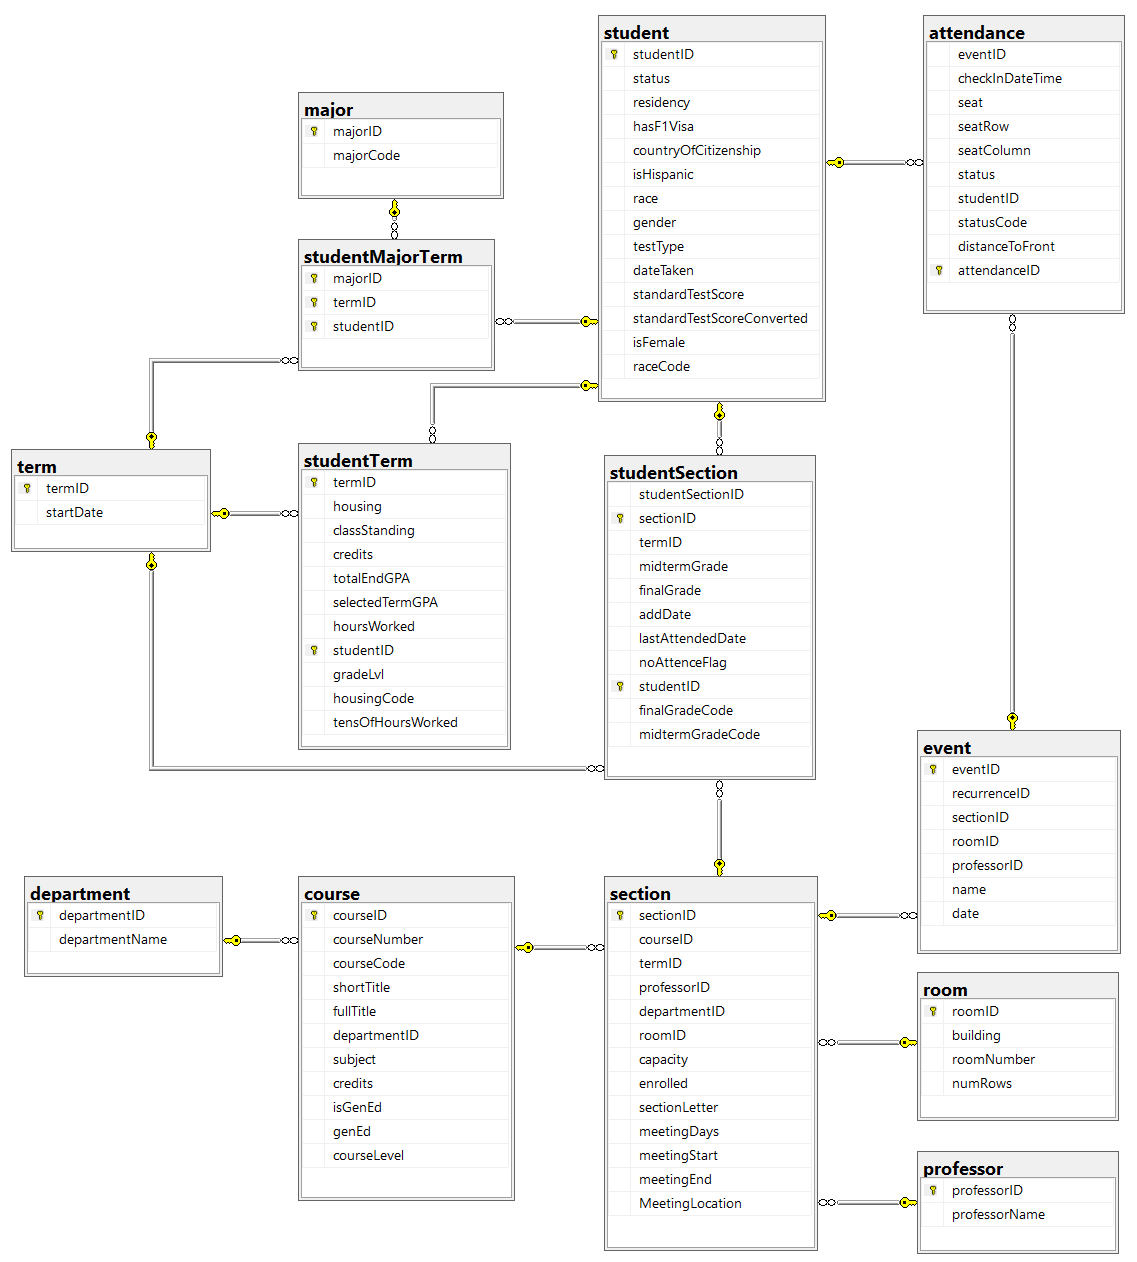
\includegraphics[width=0.92\textwidth]{figures/attendanceDBSchema.png}
  \caption{The database schema as visualized by Microsoft SQL Server Management Studio.}
  \label{fig:schema}
\end{figure}

With a data available, queries can be written. All queries were written manually to ensure quality, correctness, and diversity. For example, consider the queries in Listings \ref{lst:selectCSPhysDept} and \ref{lst:selectNursDept}. These two queries require nearly identical procedures to retrieve. Because we are interested in what the LLM's method of information retrieval

\begin{lstlisting}[
  language=SQL,
  caption={SQL query that selects professors who taught in the computing and physics departments.},
  label={lst:selectCSPhysDept}]
  select p.professorName from professor p join section s on p.professorID = s.professorID join course c on s.courseID = c.courseID join department d on c.departmentID = d.departmentID where d.departmentName = 'Computing' or d.departmentName = 'Physics';
\end{lstlisting}

\begin{lstlisting}[
  language=SQL,
  caption={SQL query that selects professors who taught in the nursing department.},
  label={lst:selectNursDept}]
  select p.professorName from professor p join section s on p.professorID = s.professorID join course c on s.courseID = c.courseID join department d on c.departmentID = d.departmentID where d.departmentName = 'Nursing';
\end{lstlisting}

\subsubsection{Database Descriptors}
We plan to provide the model with a brief description of the database it is working with. This description will include table columns and relationships as well as brief statistics about the size of those tables (to simulate) cardinality estimation.

\subsubsection{Queries}
The fundamental goal of this research is to transform SQL queries into DBMS execution plans. Therefore, each prompt must include a valid query to translate. For the purpose of consistency and quality, we utilize one university database to author several (around one hundred) SQL queries. We also collect Microsoft SQL Server's execution plan for these queries to use for comparison and evaluation.

